%!TEX root=../../template.tex
\section{\gls{DOAS}}%
\label{sec:doas}

\acrlong{DOAS} is a well established absorption spectroscopy technique
that is widely used in the field of atmospheric
studies~\cite{Platt2007}. In this section, I present a short
introduction to the field. The first part of this introduction is based
on~\cite{ValentedeAlmeida2017}, an article we have published in 2017,
marking the conclusion of the initial studies for this PhD thesis. The
second and last part refers to additional research that I have conducted
since then.

\gls{DOAS} itself is based on Lambert--Beer's law, which can be written
as \cite{Platt2007}

\begin{equation}
  \centering
  \label{eq:lambertBeer}
  I(\lambda) = I_0 (\lambda) \cdot \exp(-\sigma(\lambda) \cdot c \cdot L) \;,
\end{equation}

Where $\lambda$ is the wavelength of the emitted light; $I(\lambda)$ is
the light intensity as measured by the system; $I_{0}(\lambda)$ is the
intensity of the light as emitted by the source; and $\sigma(\lambda)$
is the absorption cross section of absorber, which is wavelength
dependent; $c$ is the concentration of the absorber we want to measure.

This law allows the definition of optical thickness
($\tau$)~\cite{Platt2007}:

\begin{equation}
      \label{eq:opticalThickness}
      \tau(\lambda) = \ln \bigg( \frac{I_{0}(\lambda)}{I(\lambda)}\bigg)
      = \sigma(\lambda) \cdot c \cdot L.
\end{equation}

In a laboratory setting, Eq.~(\ref{eq:lambertBeer})
or~(\ref{eq:opticalThickness}) can be used to directly calculate an
absorber's concentration, provided there is knowledge of  its cross
section. In the open atmosphere, however, absorption spectroscopy
techniques are far more complex. On one hand, $I_0(\lambda)$ is not
accessible since we measure from inside the medium we want to measure.
On the other hand, there are several environmental and instrumental
effects that influence measurement results. These effects include the
following~\cite{Platt2007}.

\begin{itemize}
      \item Rayleigh scattering is due to small molecules present in the
          atmosphere and is heavily influenced by wavelength (hence the
          blue colour of the
      sky).
      \item Mie scattering is caused by particles and larger molecules
          suspended in the atmosphere and is not very dependent
      on the wavelength (hence the white colour of clouds).
      \item Instrumental and turbulence effects are the instrument's
          transmissivity and atmospheric turbulence in the optical path
          also limit light intensity.
  \end{itemize}

In addition, we also have to take into account that, in the atmosphere,
there are a number of trace gases that interfere with passing light.
Another aspect worth mentioning is that our device is never pointed
directly at the light source (the Sun) but always processes light that
has been scattered at some unknown point in the optical path. This means
that the light that reaches our detector is only the scattered fraction
of the sunlight, depending on the system's position and geometry, as
well as wavelength. The expansion of Lambert--Beer's equation to include
all these effects results in Eq.~(\ref{eq:expandedLambertBeer}).

\begin{equation}
    \label{eq:expandedLambertBeer}
    \begin{aligned}
        \epsilon_\mathrm{TG}(\lambda, s)&=\sum_{i} \sigma_{i}(\lambda, s)
            \cdot c_{i}(s)\\
       I(\lambda) &= I_0(\lambda) \cdot A(\lambda, \ldots) \cdot
            S(\lambda) \cdot\\
                   &\quad\cdot \exp \left[ -\int \left[
                       \epsilon_{TG}(\lambda, s) +
                           \epsilon_{\mathrm{M}}(\lambda, s) +
                               \epsilon_{\mathrm{R}}(\lambda, s)  \right] \right] 
    \end{aligned}
\end{equation}

Where $A(\lambda, \ldots)$ is the fraction of scattered light that
reaches the device, $S(\lambda)$ represents instrumental and turbulence
effects, $\sigma_{i}(\lambda, s)$ is the absorption cross section of
absorber $i$, $c_{i}$ is the concentration of absorber $i$.
$\epsilon_{\mathrm{TG}}(\lambda, s)$ is the absorption by the $i$ trace
gases, $\epsilon_\mathrm{R}(\lambda, s)$ represents Rayleigh's
extinction coefficient and $\epsilon_\mathrm{M}(\lambda, s)$ represents
Mie's extinction coefficient. The interest of this equation lies within
the retrieval of $c_i$, a given absorber's concentration. Since the
integral is taken along the total atmospheric path of the measured
photons, and considering that their cross sections do not vary
significantly in atmospheric conditions, it is possible to define the
concept of slant column, which is of great
importance~\cite{Merlaud2013}.

\begin{equation}
      \label{eq:slantColumn}
      \mathrm{SC}_{i} = \int c_{i}(s)\mathrm{d}s
\end{equation}

This quantity, as Eq.~(\ref{eq:slantColumn}) shows, equals the integral
of an individual absorber's concentration along the atmospheric optical
path of relevance. Now, without knowledge of $I_{0}(\lambda)$, these
equations cannot give us absolute concentration values. We can, however,
use another scattered light spectrum as reference in
Eq.~(\ref{eq:opticalThickness}). Instead of absolute densities, this
will yield relative changes in the atmosphere. We thus arrive at
Eq.~(\ref{eq:relativeOpticalThickness}).

\begin{equation}
    \label{eq:relativeOpticalThickness}
    \begin{aligned}
        \ln\Bigg( \frac{I_\mathrm{ref}}{I}(\lambda) \Bigg) &= 
            \ln\Big( \frac{A_\mathrm{ref}}{A}(\lambda,\ldots) \Big) + \ln\Big( 
                \frac{S_\mathrm{ref}}{S}(\lambda) \Big) \nonumber\\
                                                           &+  \sum_{i} 
            (\sigma_{i}(\lambda) \cdot \Delta \mathrm{SC}_{i}(\lambda)) + 
                \Delta \tau_\mathrm{M}(\lambda) \nonumber\\
    \end{aligned}     
\end{equation}

Where $\Delta \mathrm{SC}_{i}$  is the relative slant column of absorber
$i$; $\Delta \tau_\mathrm{M}$  is the relative Mie scattering term,
integrated to its optical thickness; and $\Delta \tau_\mathrm{R}$ is the
relative Rayleigh scattering term, integrated to its optical thickness.
This is where the principle of DOAS is applied. Instrument features,
scattering and other atmospheric effects have broad absorption spectral
profiles, which vary slowly with wavelength. Several trace absorbers
have narrow and rapidly varying spectral signatures in at least a small
section of the spectrum. By using Eq.~(\ref{eq:separation}), we can
separate these contributions \cite{Danckaert2015}.

\begin{equation}
      \label{eq:separation}
      \sigma(\lambda) = \sigma{'}(\lambda) + \sigma_{0}(\lambda)
\end{equation}

Here, the broad part of the optical thickness ($\sigma_{0}(\lambda)$)
can be separated from the narrow part ($\sigma{'}(\lambda)$ --
differential) by approximating it by a low-order polynomial, resulting
in Eq.~(\ref{eq:DOAS}).

\begin{equation}
    \label{eq:DOAS}
    \begin{aligned}
        \ln\left( \frac{I_\mathrm{ref}}{I}(\lambda) \right) &= \sum_{i = 1}^{n} \sigma_{i}{'}(\lambda) 
            \cdot \Delta \mathrm{SC}_{i} + \sum_{j = 0}^{m} a_{j} \cdot \lambda^{j}
    \end{aligned}
\end{equation}

Where $\sum_{i = 1}^{n} \sigma_{i}{'}(\lambda) \cdot \Delta SC_{i}$ is
the differential part (narrowband, rapidly varying with wavelength) and
$\sum_{j = 0}^{m} a_{j} \cdot \lambda^{j}$ is a low-order polynomial,
used to remove the broadband spectral features resulting from
atmospheric and instrumental phenomena.

In practice, the mathematical solving of Eq.~(\ref{eq:DOAS}) is not
enough since it does not account for the Ring effect or the
non-linearities that result from stray light and wavelength shift in
measured and cross-section spectra.

The Ring effect is a consequence of rotational Raman scattering:
molecules in the atmosphere do not absorb photons in a purely elastic
(Rayleigh scattering) fashion. A small portion of the light--matter
interaction is in fact inelastic \cite{Brinkmann1968,Merlaud2013}. This
changes the light source frequencies as seen from the detector. This
phenomenon was first noticed by Grainger and Ring in 1962. At the time,
they noticed that the well-known Fraunhofer lines would slightly change
when one  observed them by using moonlight instead of scattered daylight
\cite{GRAINGER1962}. Mathematically, the Ring effect is introduced into
the \gls{DOAS} expressions as a synthetically produced pseudo-absorber.

Up until this point, the \gls{DOAS} problem can be solved by a system of
linear equations of the form displayed in
Equation~\ref{eq:linearSystem}.

\begin{equation}
    \label{eq:linearSystem}
    \tau = A \cdot X
\end{equation}

$A$ is an $m \times n$ matrix. Its columns are the differential
cross-sections fot he measurement target gas, $\sigma_{i}^{'}(\lambda)$,
and the wavelength powers ($\lambda$ ,$\lambda^2$, $\lambda^3$, \ldots)
according to the polynomial used for the broadband extraction described
above, $P(\lambda)=\sum_{j=0}^{m} a_{j}\lambda^{j}$. The lines of matrix
$A$ are the wavelength window of study, as \emph{seen} by the
spectrometer used in the experiment. This leads to there being many more
lines than columns in $A$. The system is thus overdetermined. Solving it
requires the use of numerical approximations, and the most common
approach is a least-squares approximation, in which the best solution
minimises $\chi^2=\left[\tau - A \cdot X\right]\left[\tau - A \cdot
X\right]^T$. The upper script $T$ used in this expression denotes the
transpose of the preceding matrix~\cite{Merlaud2013, Platt2007}.

A crude \gls{DOAS} algorithm might not go any forward. In effect, this
is precisely the approached followed in~\cite{ValentedeAlmeida2017} for
smoke detection using machine learning techniques. A more refined
measurement, aimed at quantification of the target trace gases and not
at determining the presence of a particular type of atmospheric event
requires an additional consideration, and some more algorithmic steps.
There are in fact some non-linearities in the complete retrieval
process. These non-linearities are not retrievable through linear
algorithms alone. These non-linear effects present themselves as shifts,
stretches and offsets in the measured signal. They do not directly
change the dependent variable values (i.e., the radiance), but instead
"move" the scale of the independent variable (i.e., the wavelength).
Therefore, linear approximations such as least-squares minimisation are
not sensitive to them. A non-linear approximation algorithm such as
Levenberg--Marquardt~\cite{Press2007} can be used, and the expression
that is being solved is presented in Equation~\ref{eq:DOAS_nonLinear}.

\begin{equation}
    \label{eq:DOAS_nonLinear}
    \begin{aligned}
        \ln \left( \frac{I_\mathrm{ref}(\lambda)}{I(\lambda +
            \mathrm{shift}) + \mathrm{offset}} \right) &= \sum_{i=1}^{n}
                \sigma_{i}{'}(\lambda) \cdot \Delta \mathrm{SC}_{i} + 
                    \sum_{j=0}^{m} a_{j} \cdot \lambda^{j}
    \end{aligned}
\end{equation}

Programming-wise, solving these equations is an iterative two-stage
process, which runs until one of the following typical stop criteria are
met.

\begin{description}
    \item[Maximum iteration number:] This is a self-explanatory
        criterion. It limits the number of times the algorithm's cycle
        can run; 
    \item[Minimum improvement threshold:] As the algorithm proceeds,
        this criterion ensures that it progresses in the correct
        direction, i.e., minimising $\chi^2$;
    \item[Minimisation target:] If $\chi^2$ becomes lower than this
        given threshold, the cycle is terminated. 
\end{description}

The cycle begins by the determination of the concentration values of the
target trace gases and the $\chi^2$ score is calculated. The wavelength
window is shifted, stretched and offset according to the initial
conditions. The $\chi^2$ is re-calculated and compared to the previous
value. This cycle is iteratively repeated in the best minimisation
direction until any of the stop criteria are met and the cycle is
terminated. The algorithm is illustrated (simplified) in
Figure~\ref{fig:doas_non_linear}.

\begin{figure}[htpb]
    \centering
    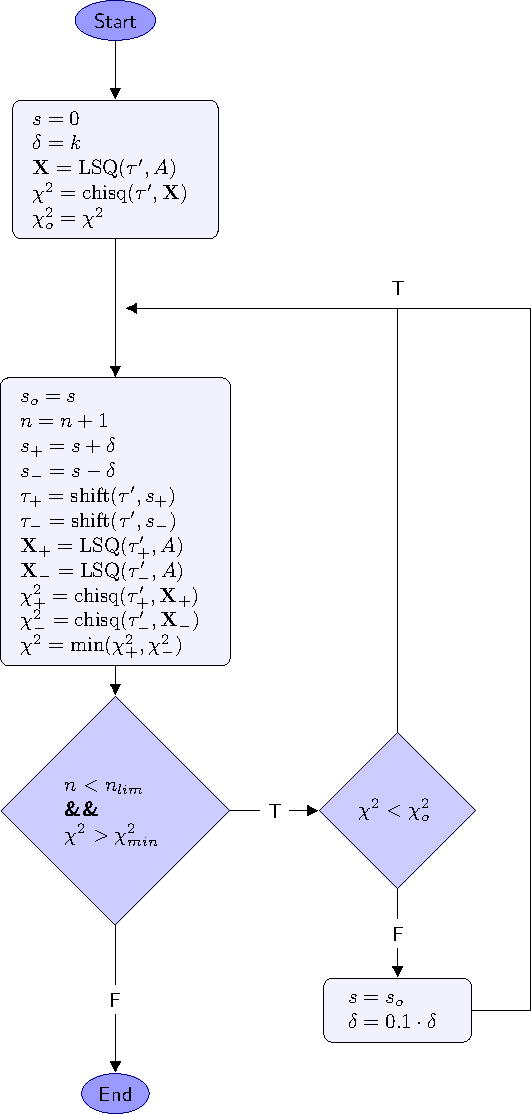
\includegraphics[width=0.4\textwidth]{tikz/doasFlowchart/doasFlowchart.pdf}
    \caption{Simplified schematic flowchart of the \gls{DOAS} algorithm,
    including the non-linear part.}
    \label{fig:doas_non_linear}
\end{figure}

\subsection{ Types of \gls{DOAS} experiments}%
\label{sub:doas_categories}

There are two main families of \gls{DOAS} assemblies, with different
goals and capabilities:

\begin{itemize}

        \item Active systems, of which a simple illustration is
            presented in Fig.~\ref{fig:activeSmall}, are characterized
            by relying on an artificial light source for their
            measurements. A spectrometer at the end of the light path
            performs spectroscopic detection. Active DOAS techniques are
            very similar to traditional in-lab absorption spectroscopy
            techniques \cite{Platt2007};

            \begin{figure}[htb]
                \centering
                \includegraphics[width=.8\textwidth]{img/pdf/amt-2016-314-f02.pdf}
                \caption{Active DOAS schematic.}\label{fig:activeSmall}
              \end{figure}

        \item Passive DOAS techniques, illustrated in
            Fig.~\ref{fig:passiveSchematic}, use natural light sources,
            such as the Sun and the moon, in their measurement process.
            An optical system is pointed in certain elevation and
            azimuth angles and sends the captured light into a
            spectrometer, connected to a computer. The system returns
            the total value of the light absorption in its
            path~\cite{Platt2007,Merlaud2013}.

              \begin{figure}[htb]
                  \centering
                  \includegraphics[width=.8\textwidth]{img/png/amt-2016-314-f03.png}
                  \caption{Passive DOAS schematic.}\label{fig:passiveSchematic}
              \end{figure}
\end{itemize}

Within the two main \gls{DOAS} families, there are several types of
possible experiment. Differences in the design of these assemblies
originate from a number of different target requirements. Active or
passive applications can differ with relation to their intended spectral
range, light throughput or resolution, among others.

In active experiments, the choice of the light source is the most
critical aspect of the whole experimental design. Active \gls{DOAS}
light sources must be stable, have a very high throughput (these
experiments are often conducted over long optical paths) and must have
an adequate cost to purchase, maintain and operate. This is especially
true in long-running experiments, which must remain working for months
or even years. Moreover, the spectral range of the emitted light is also
of central importance, because most trace gases have very particular
spectral cross sections. The spectral structure of the emitted light is
also an important feature to consider, for similar reasons.

The sun and the moon are the two most important light sources when it
comes to passive \gls{DOAS} applications. Sunlight can be used directly
or after a scattering event, the latter being the more common. In these
experiments, instead of pointing directly at the sun, the collector is
pointed at a certain point in the atmosphere, entering the system after
it has been scattered. There are many possible geometries to a scattered
sunlight \gls{DOAS} experiment. Some of them are schematically
represented in Figure~\ref{fig:doasTypes}.

\begin{figure}[htpb]
    \centering
    \begin{subfigure}[b]{.475\textwidth}
        \centering
        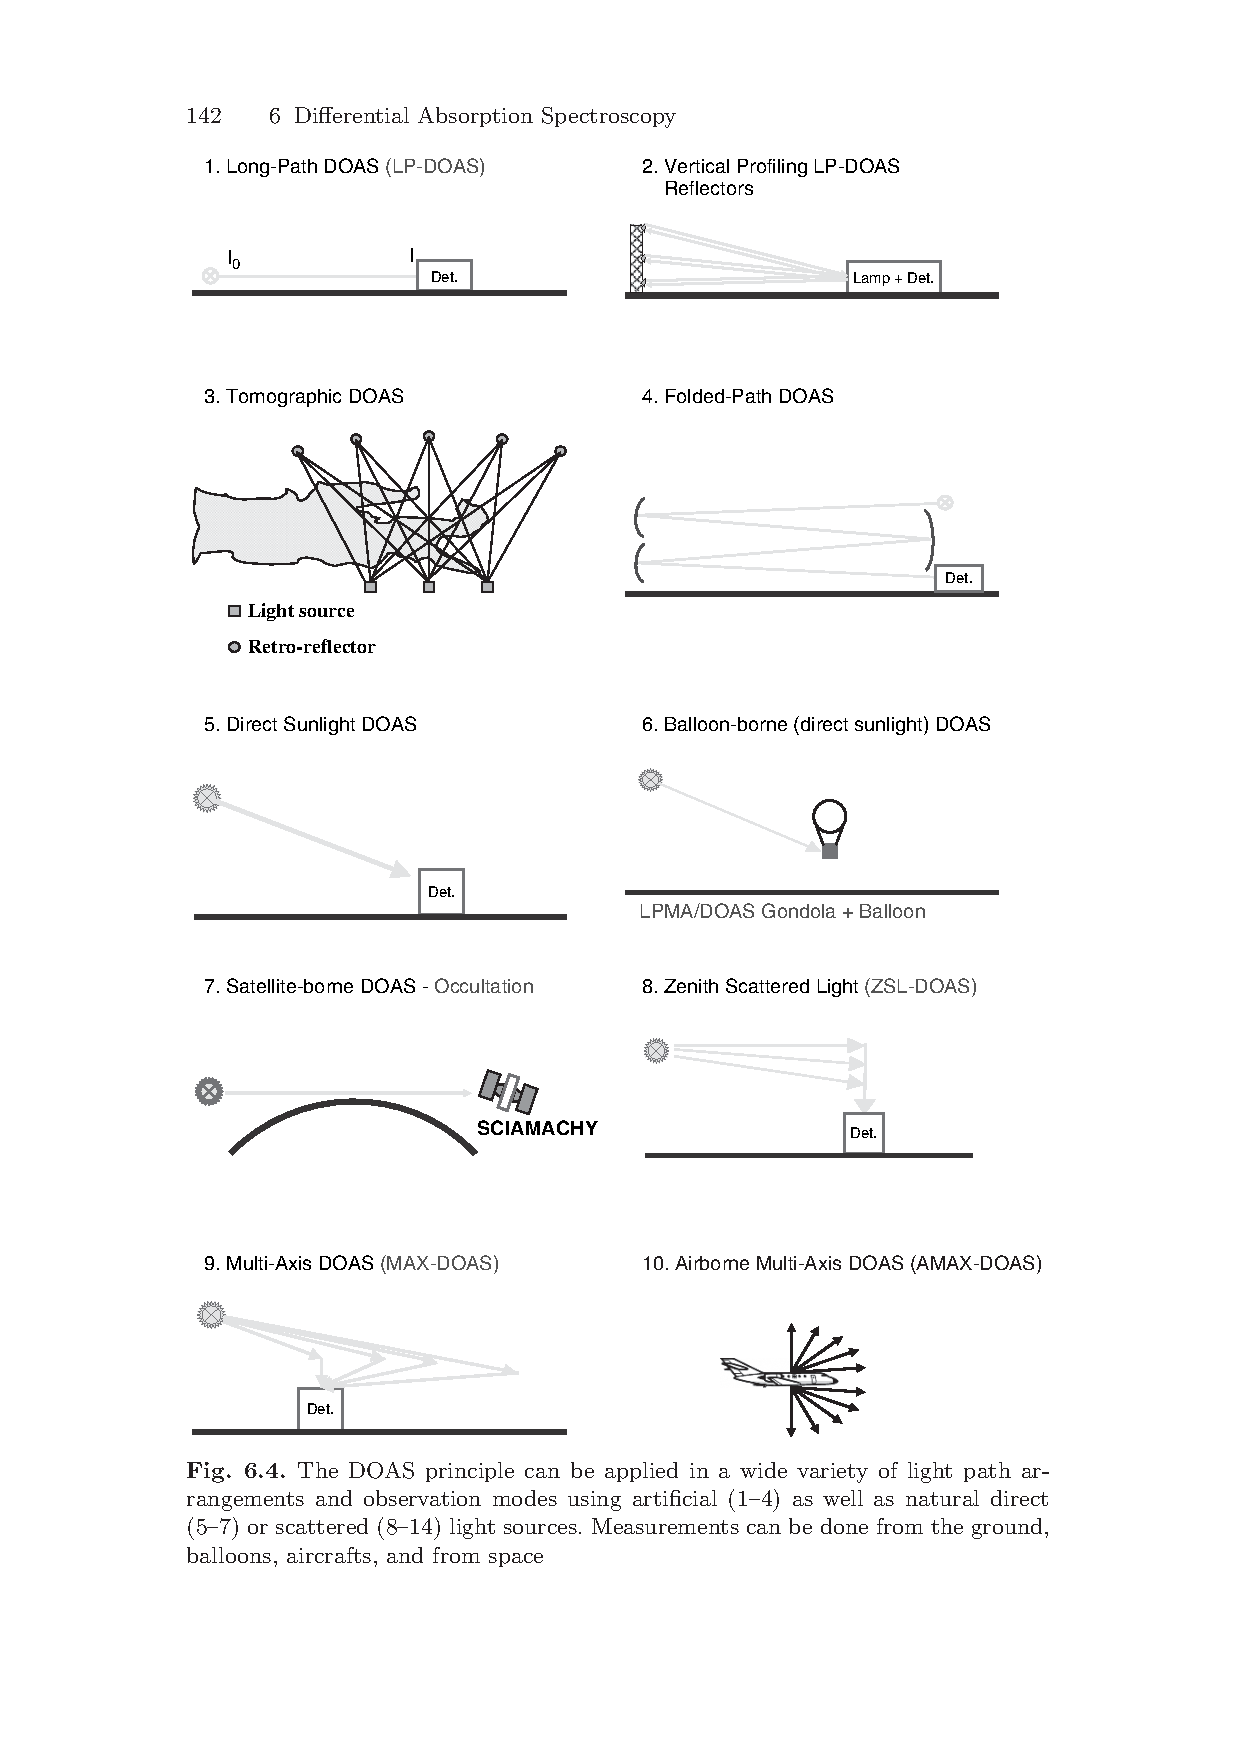
\includegraphics[trim=10.8cm 10cm 4.5cm
        16.9cm, clip, width=\textwidth]{img/pdf/zenithMaxAMax.pdf}
        \caption{Zenith Scattered Sunlight}
        \label{fig:zsldoas}
    \end{subfigure}
    \hfill
    \begin{subfigure}[b]{.475\textwidth}
        \centering
        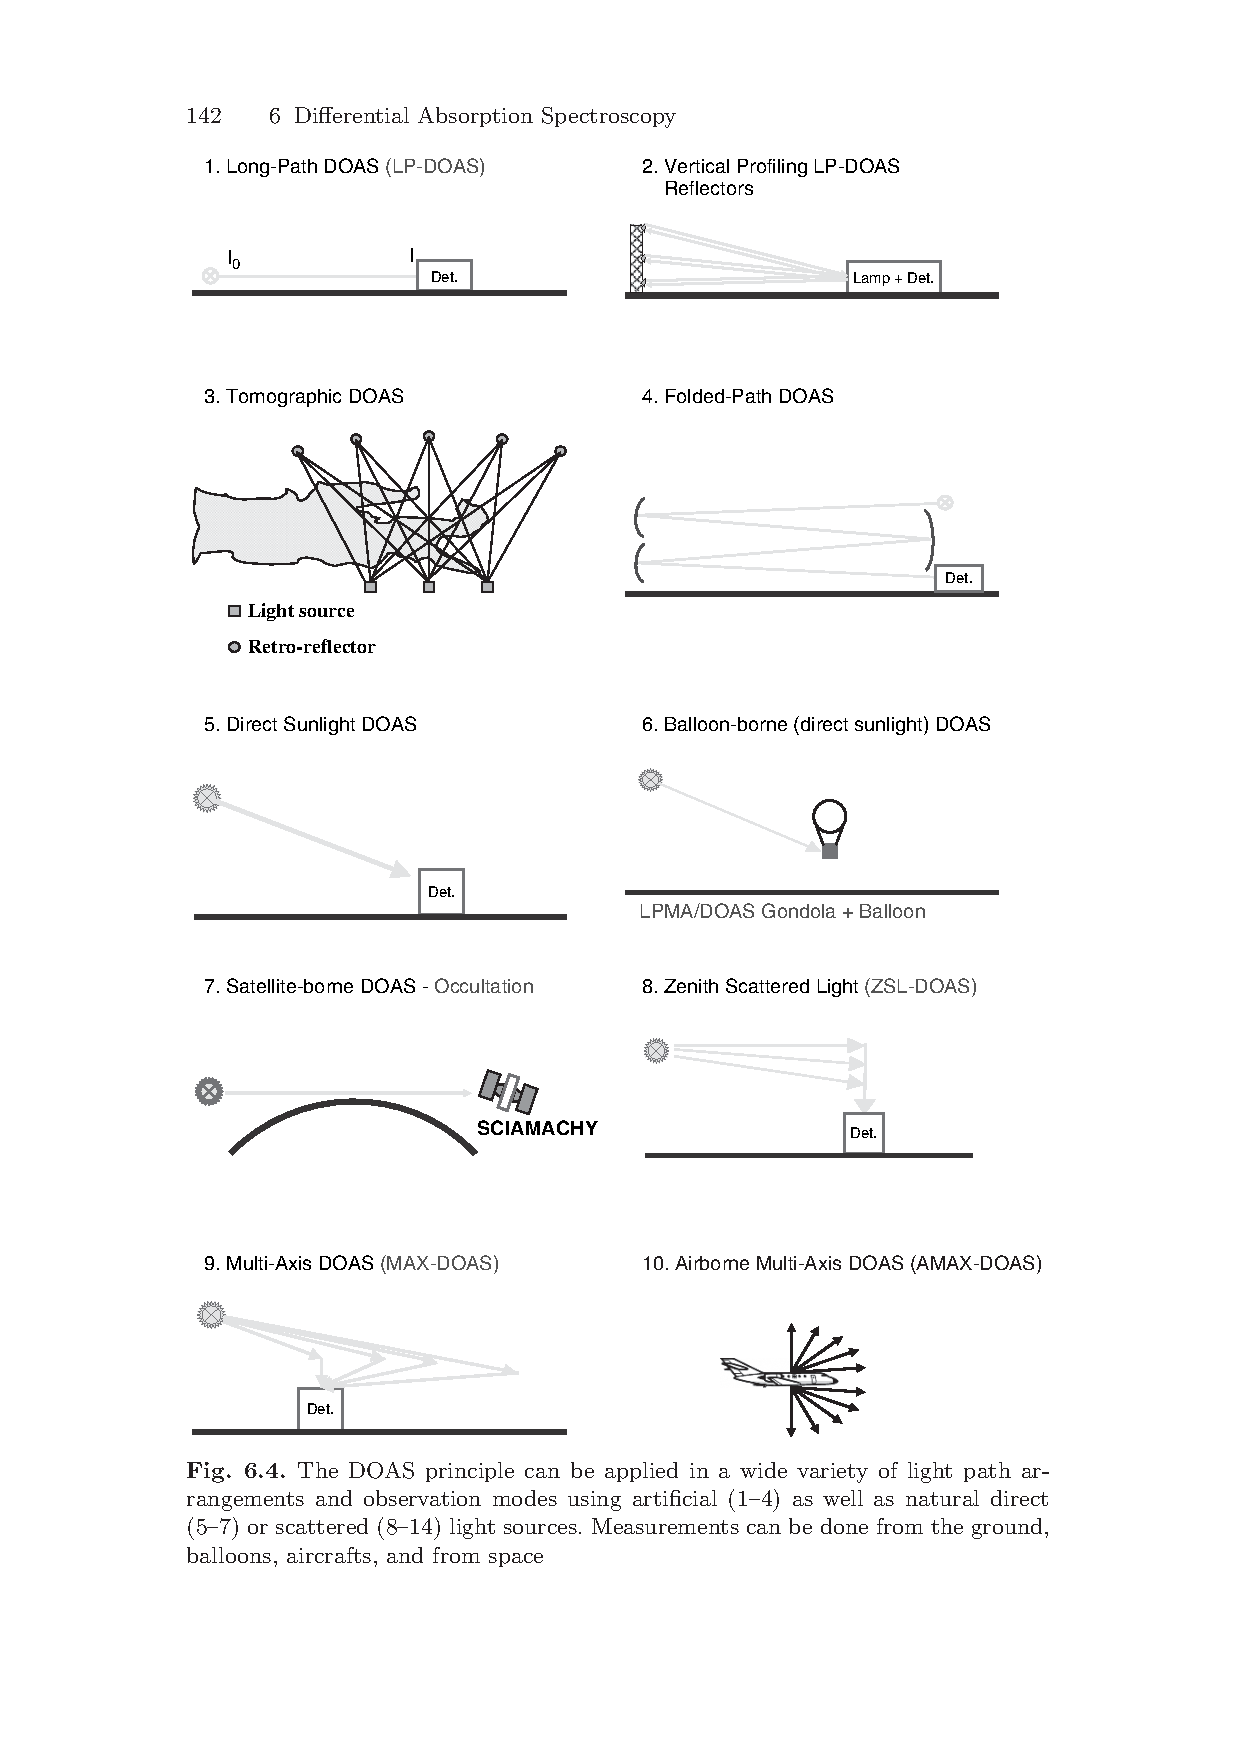
\includegraphics[trim=3cm 5.3cm 12cm
        21.7cm, clip, width=\textwidth]{img/pdf/zenithMaxAMax.pdf}
        \caption{\gls{maxdoas}}
        \label{fig:maxdoas}
    \end{subfigure}
    \hfill
    \begin{subfigure}[b]{.475\textwidth}
        \centering
        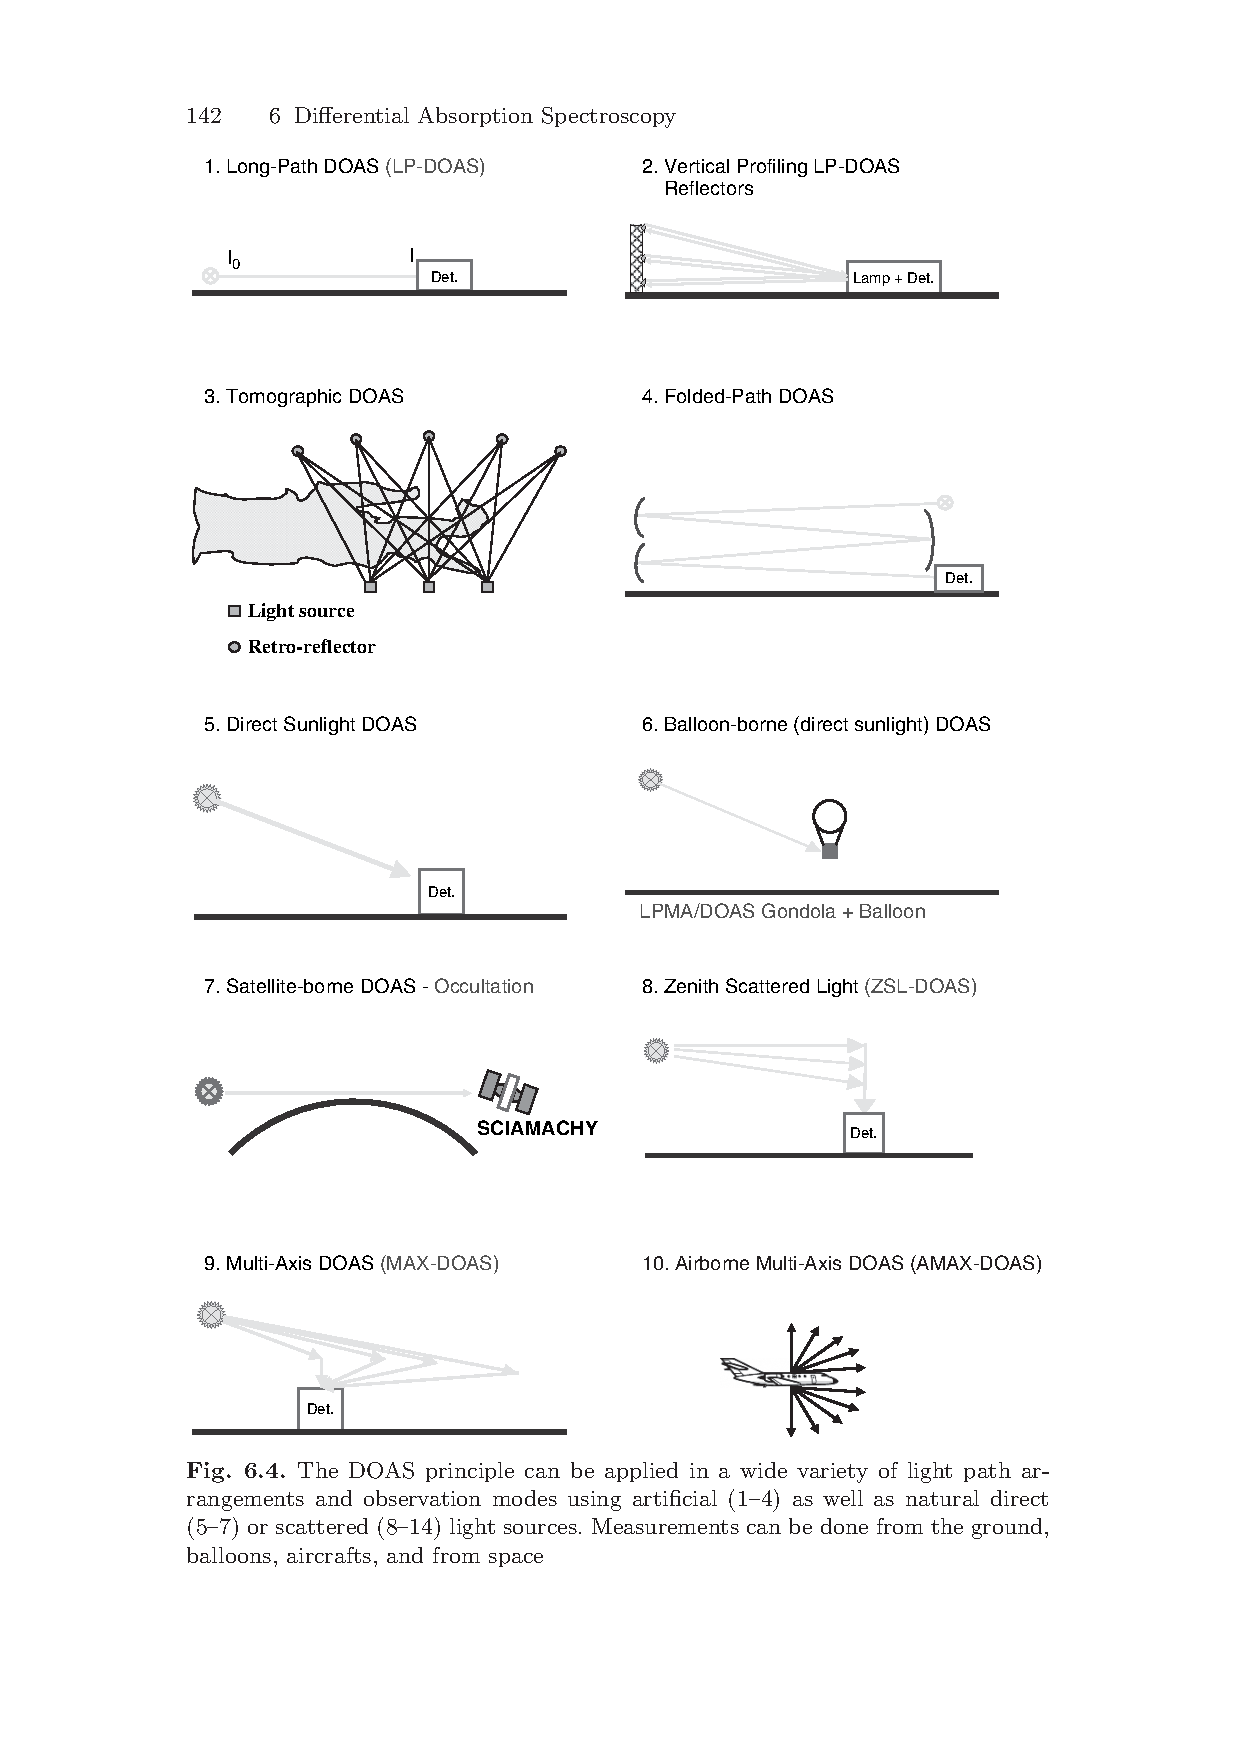
\includegraphics[trim=10.8cm 5.3cm 4.5cm
        21.7cm, clip, width=\textwidth]{img/pdf/zenithMaxAMax.pdf}
        \caption{Airborne \gls{maxdoas}}
        \label{fig:amaxdoas}
    \end{subfigure}
    \hfill
    \begin{subfigure}[b]{.475\textwidth}
        \centering
        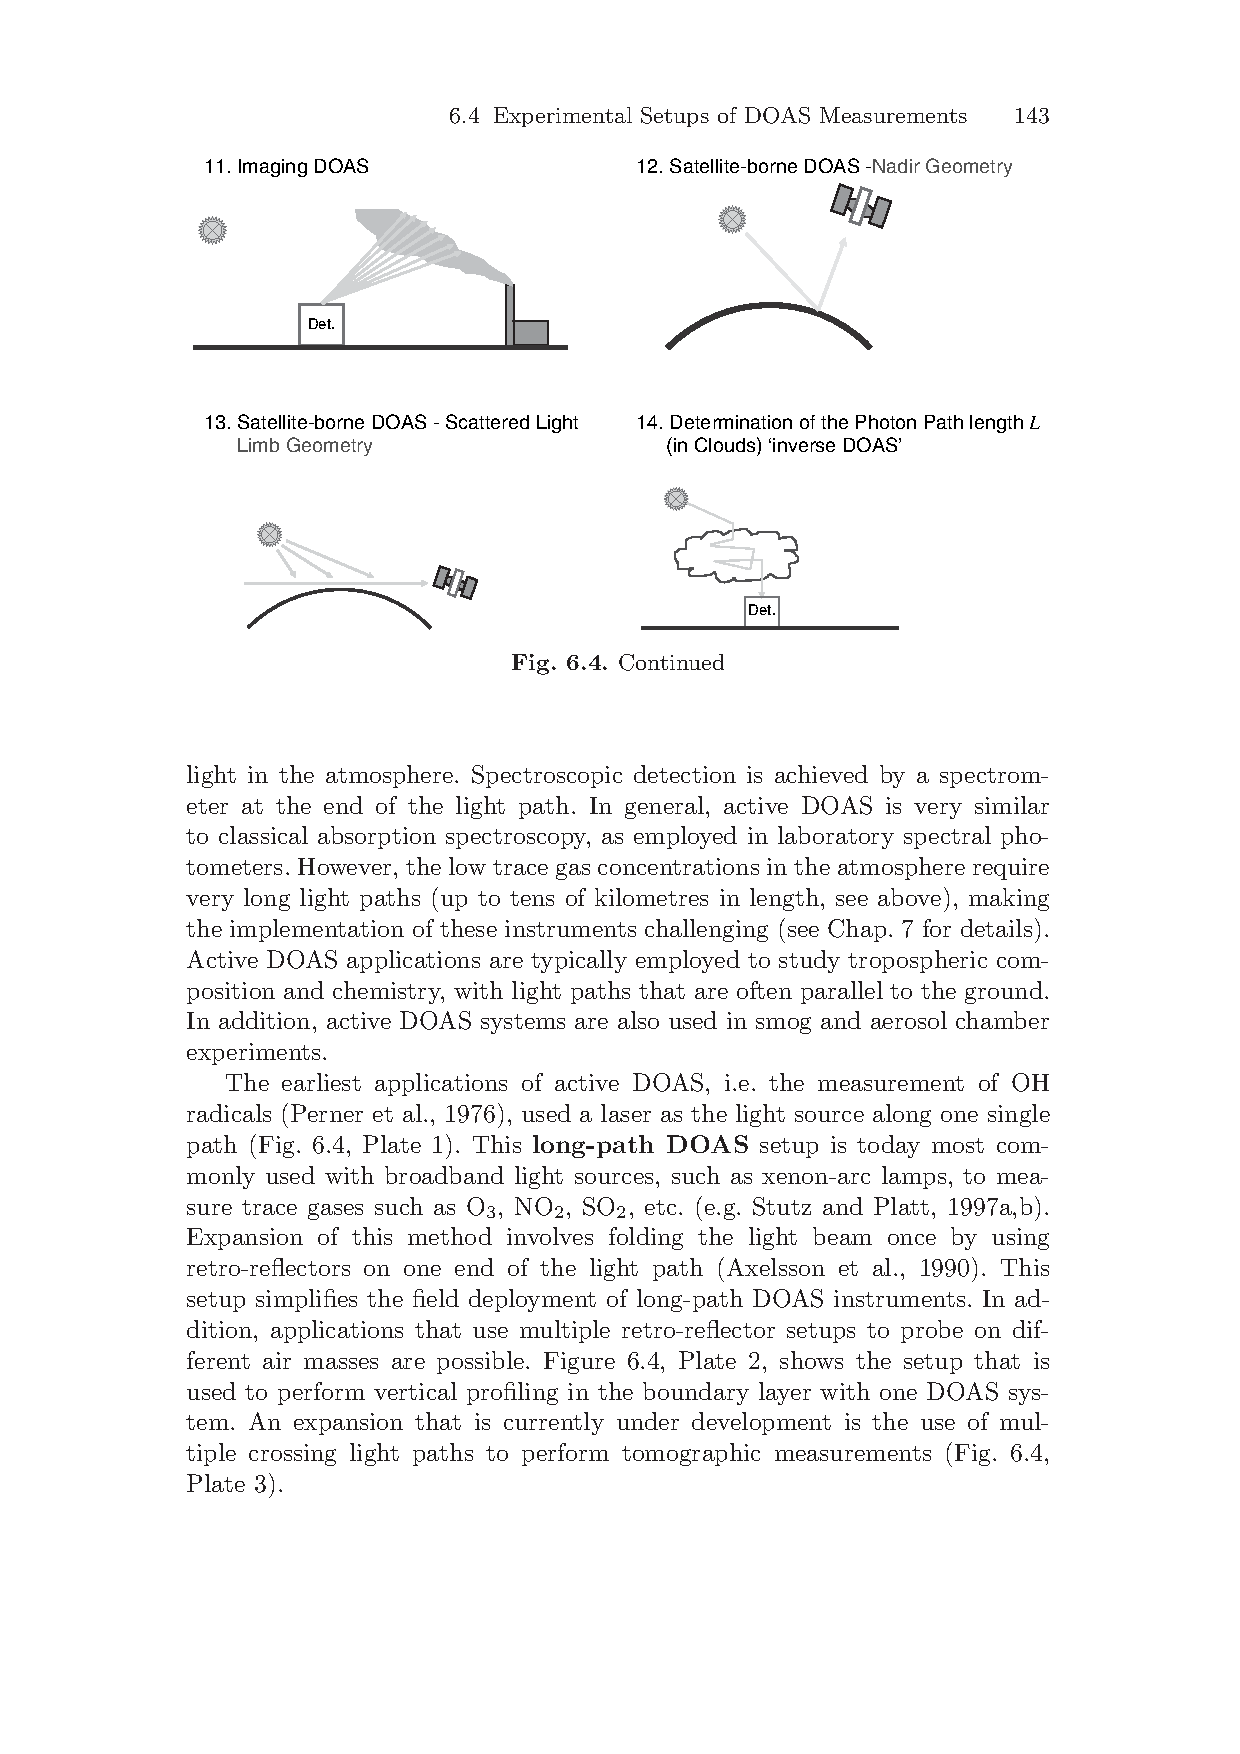
\includegraphics[trim=3cm 23.7cm 12cm
        3cm, clip, width=\textwidth]{img/pdf/imaging.pdf}
        \caption{Imaging \gls{DOAS}}
        \label{fig:imagingDoas}
    \end{subfigure}
    \caption{Several examples of possible passive \gls{DOAS} experiment
    geometries. All these examples use only the light from an
    astronomical source to detect many atmospheric trace gases. All
    these examples were taken from~\cite{Platt2007}.}
    \label{fig:doasTypes}
\end{figure}

Although instrumentally simpler than their active counterpart, passive
\gls{DOAS} applications require more care in the retrieval process. In
this kind of application, light sources are extremely far away.
Additionally, they are normally highly structured. This means that one
has to be extremely mindful when using it for the retrieval of small
concentration changes. In addition to this, there is always the need to
convert the system's direct measurement, a column density, into vertical
densities. Since in scattered sunlight measurements, the optical path is
impossible to calculate in a precise manner, this requires the use of
complex radiative transfer models~\cite{Platt2007, Frins2006}.

\subsubsection{Satellite Measurements}%
\label{ssub:satellite_measurements}

One particularly interesting use of passive \gls{DOAS} are satellite
measurements. There are three types satellite \gls{DOAS} experiments:
\begin{description}
    \item[Occultation measurements:] this is a direct sunlight
        measurement. Light comes from the sun and traverses the Earth's
        atmosphere in a tangential manner before entering the
        satellite's light collector;

        \begin{figure}[htpb]
            \centering
            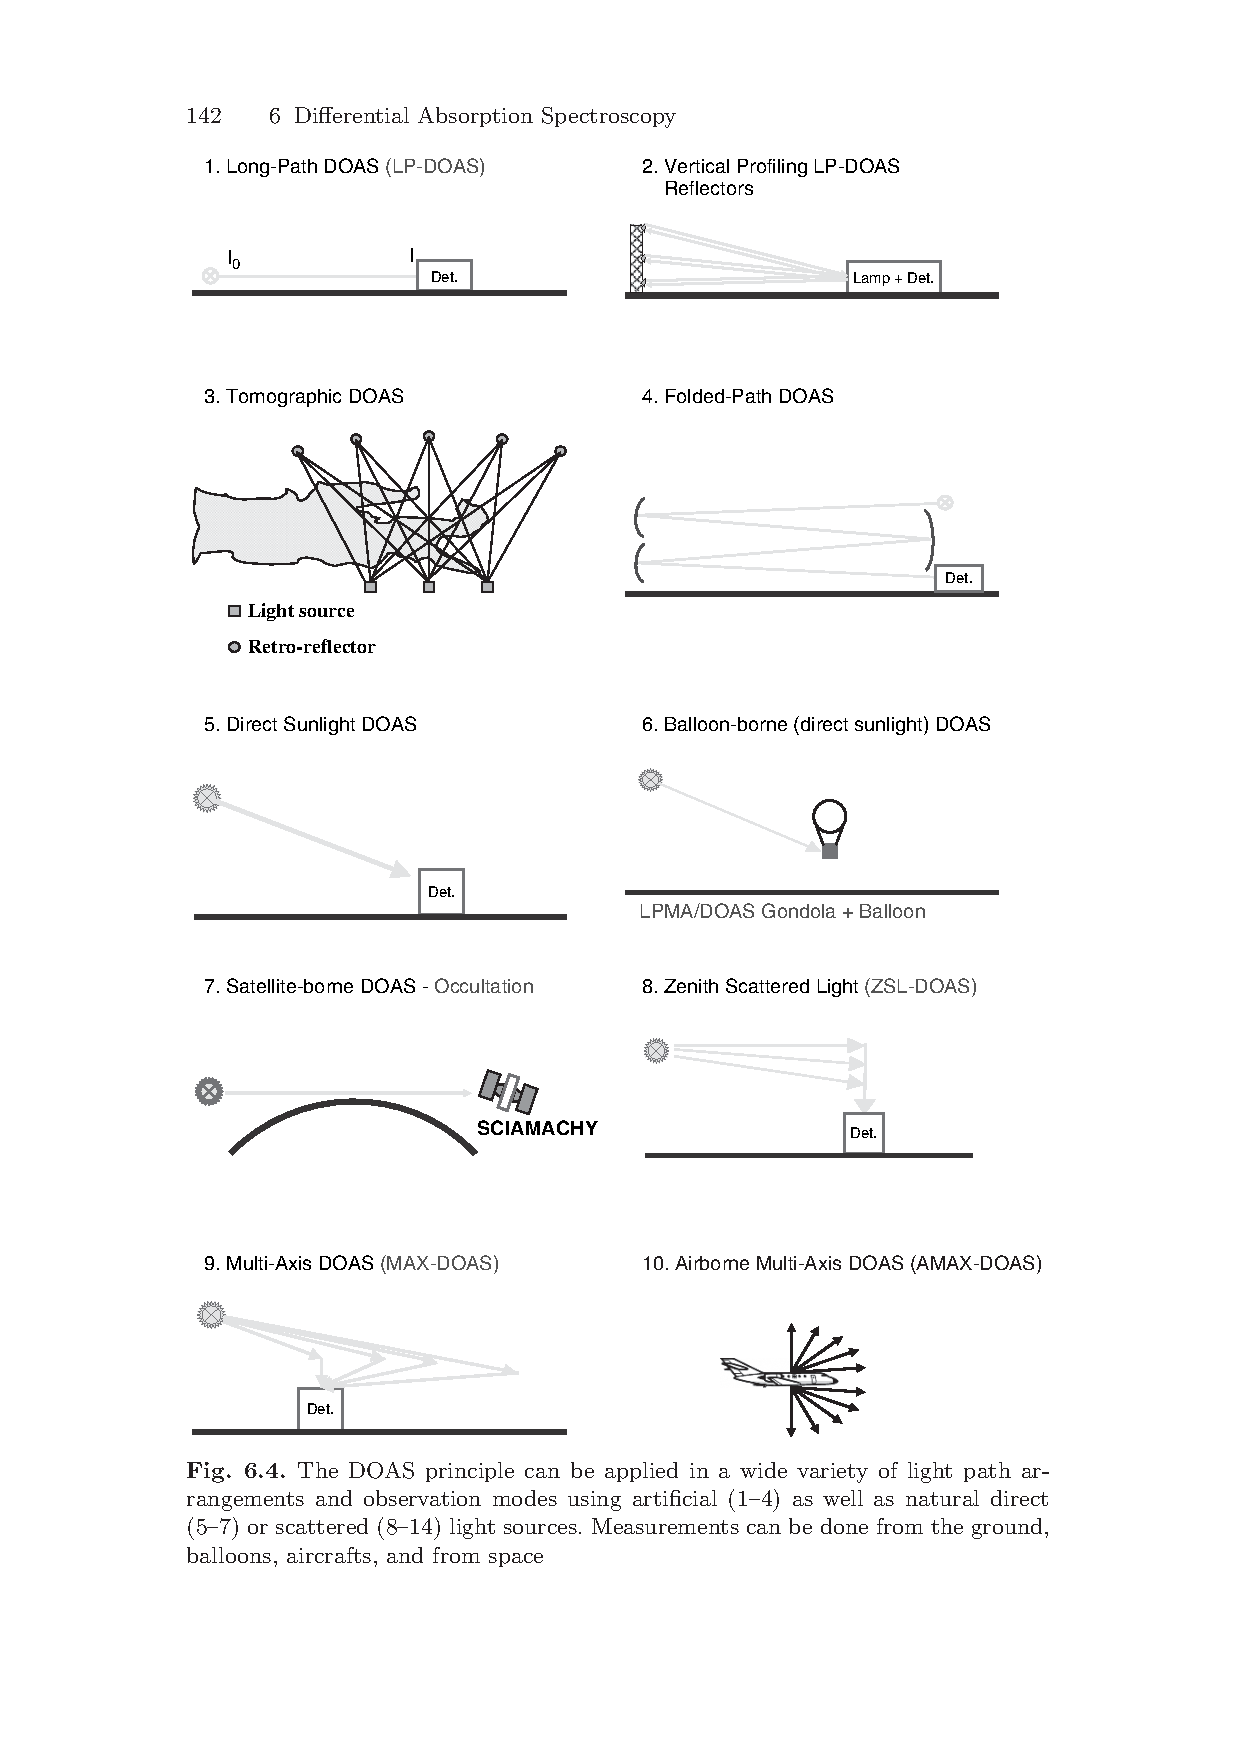
\includegraphics[trim=3cm 10cm 10.5cm
            18cm, clip, width=\textwidth]{img/pdf/zenithMaxAMax.pdf}
            \caption{Occultation measurement schematic
            representation~\cite{Platt2007}}
            \label{fig:occultation}
        \end{figure}

    \item[Limb:] a scattered sunlight measurement, in which the
        collector is pointed towards the Earth, at an angle. Light
        reaches the detector after being scattered in the atmosphere,
        the ground, or both;
        \begin{figure}[htpb]
            \centering
            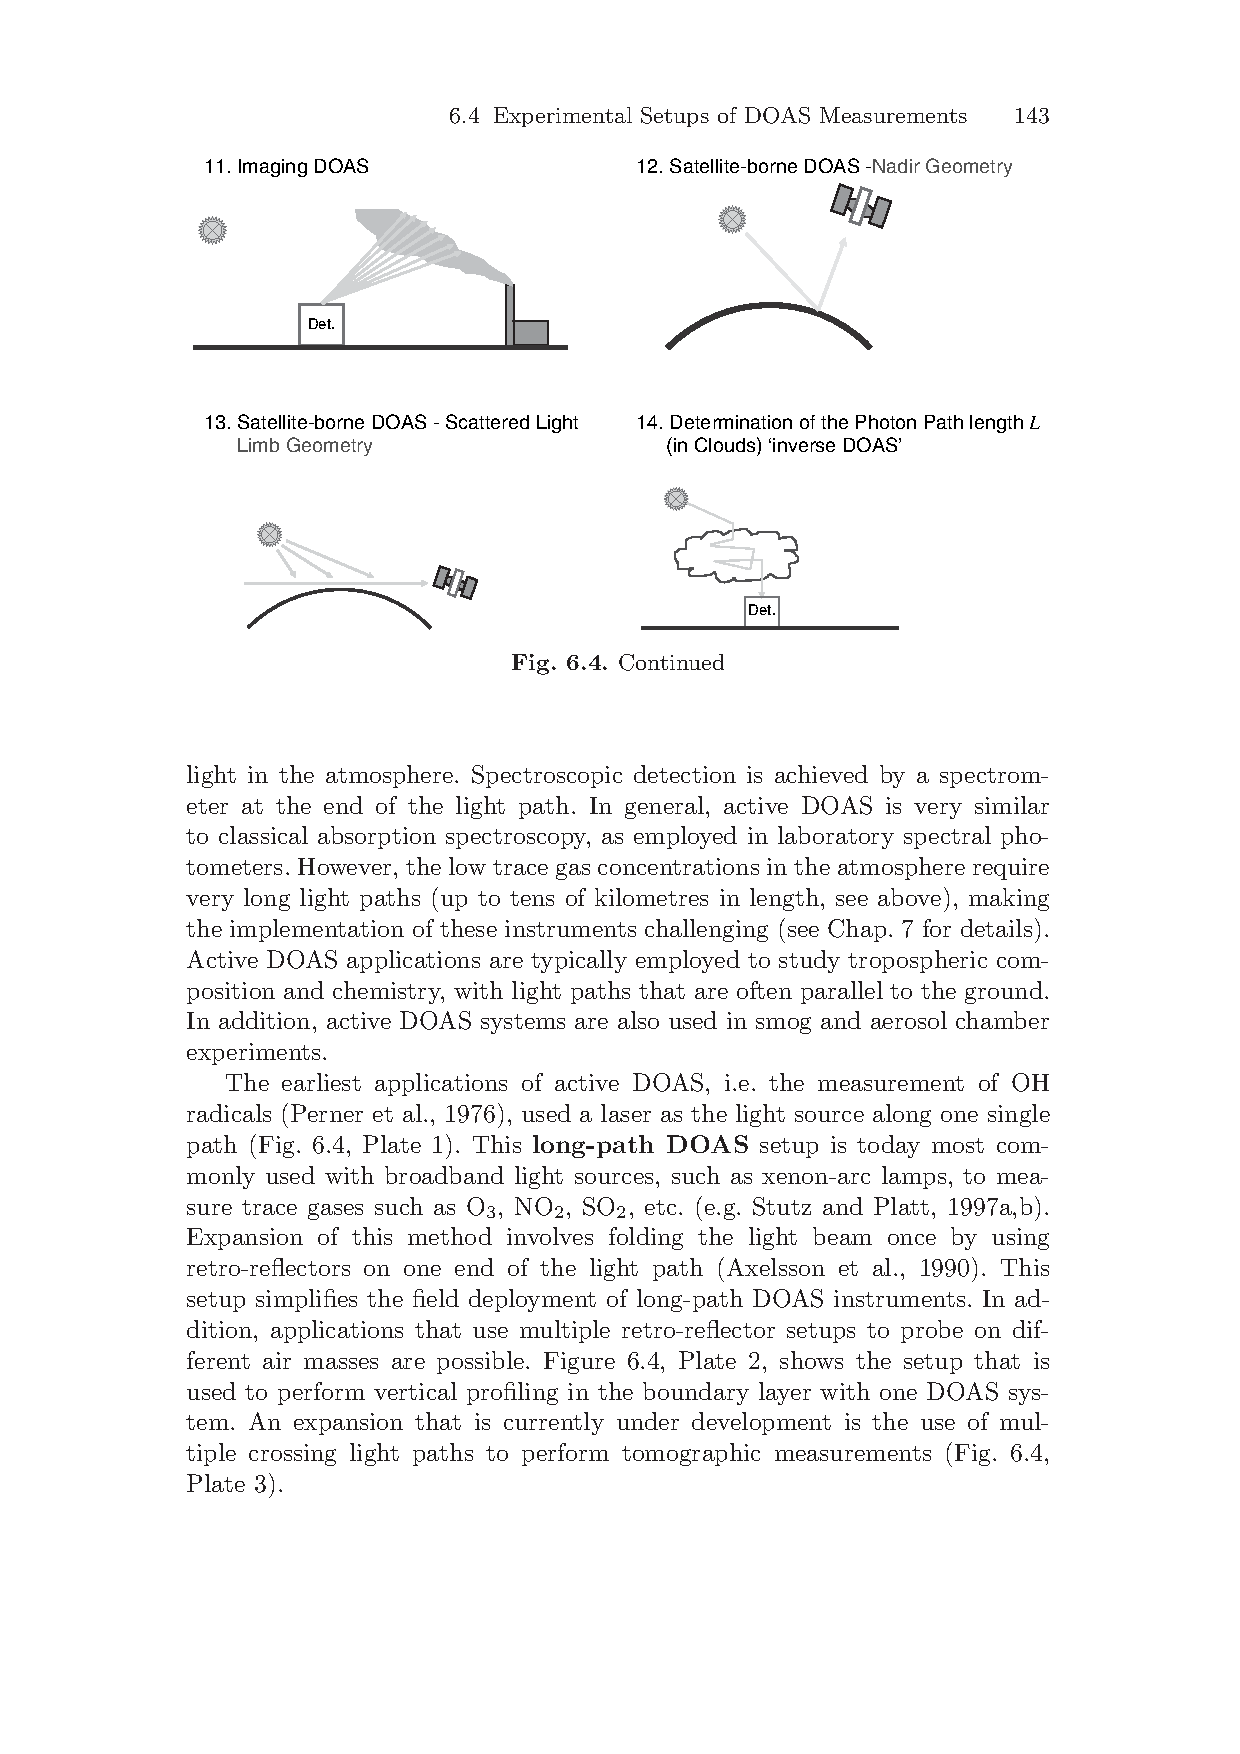
\includegraphics[trim=3cm 19cm 12cm
            8.5cm, clip, width=\textwidth]{img/pdf/imaging.pdf}
            \caption{Schematic representation of the limb satellite
            measurement geometry.}
            \label{fig:limb}
        \end{figure}
    \item[Nadir:] this is the most common measurement geometry for
        satellite experiments. In this mode, light that gets reflected
        off the Earth's surface is captured by the collecting device,
        while it is pointing directly down.
        \begin{figure}[htpb]
            \centering
            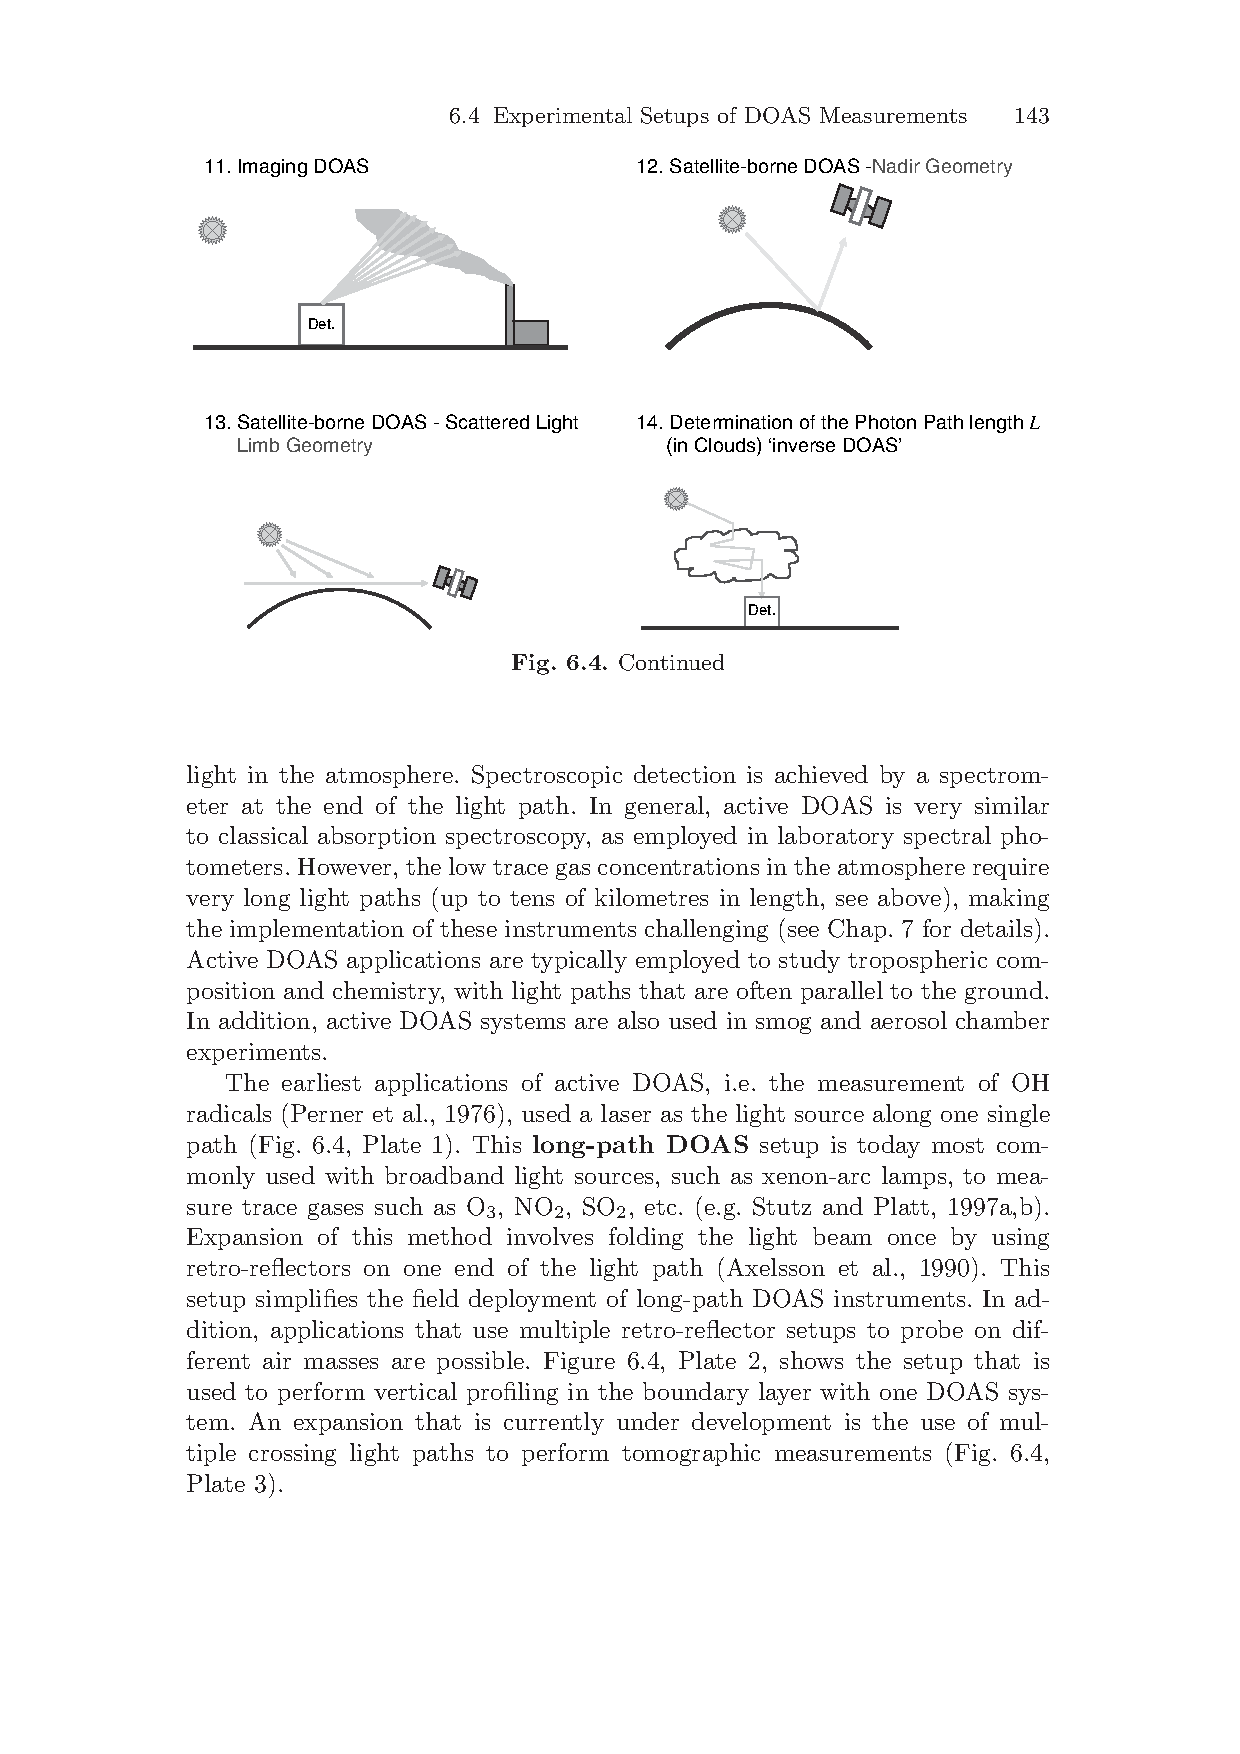
\includegraphics[trim=10cm 23.7cm 5cm
            3cm, clip, width=\textwidth]{img/pdf/imaging.pdf}
            \caption{Schematic representation of the nadir satellite
            measurement geometry.}
            \label{fig:nadir}
        \end{figure}
\end{description}

Satellite based \gls{DOAS} measurements have also been important because
they have given rise to new trace gas retrieval techniques. Through
them, new trace gases, previously unreachable through \gls{DOAS} have
been quantified on a global level, such as carbon monoxide through
\gls{wfm}~\cite{Buchwitz2000, Buchwitz2004}.

\gls{wfm} is a trace gas column retrieval algorithm, developed in the
beginning of the 21\textsuperscript{st} century, with the main goal of
determining the total columns of gases such as \gls{co}, \gls{h2o} or
\gls{co2} from satellite nadir data~\cite{Buchwitz2004}. Instead of
using literature-obtained cross-section data for each target trace gas,
the \gls{wfm} approach uses weighing functions, calculated through the
application of a radiative transfer model, such as
SCIATRAN~\cite{Rozanov2002}. Still, the retrieval is based on a
fitting process. Equation~\ref{eq:wfmdoas}, adapted
from~\cite{Buchwitz2000, Buchwitz2004} can be called the \gls{wfm}
equation.

\begin{equation}
    \centering
    \left \lVert \ln I_{i}^{obs}(\bm{V^t}) - \left[ \ln
            I_{i}^{mod}(\bm{\bar{V}}) +
        \sum_{j=1}^{J} \frac{\partial \ln I_{i}^{mod}}{\partial V_{j}}
        \middle \vert_{\bar{V_{j}}} (\hat{V_{j}} - \bar{V_{j}}) +
        P_{i}(a_m)
    \right] \right\rVert^{2} = \left \lVert RES \right \rVert^2
    \rightarrow min
    \label{eq:wfmdoas}
\end{equation}

In Equation~\ref{eq:wfmdoas}, $I_{i}^{obs}$ is the observed
sun-normalised radiance (the ratio between a nadir radiance measurement
and solar irradiance) for the center wavelength $\lambda_i$ of detector
pixel number $i$. $\bm{V}$ are the vector that have vertical columns as
their components. These can be true, $V^t$, modelled, $\bar{V_j}$, or
approximated, $\hat{V_j}$. The true columns are unknown as we only have
the radiance value and not the things on which it depends, modelled
vertical columns are taken from the literature (they are climatological
values) and $\hat{V_j}$ are one of the fitting parameters. The other
being $a_m$, the low order polynomial ($P$) coefficients. $RES$ is
the fit residuum, which is minimised for the fitting. 

\section{Important Notes on \gls{DOAS} in practice}%
\label{sec:important_notes_on_doas_in_practice}

Theoretically, the procedure described in Section~\ref{sec:doas} would
be enough to obtain the target trace gas concentrations. In practice,
this is an over-simplification. There are several additional required
steps, most of them concerning a certain conditioning that one has to
apply to both the collected and literature spectral signals.

\subsection{Cross section conditioning}%
\label{sub:cross_section_conditioning}

Unless conditions are absolutely stable, and one is able to record all
data with the same device, which is impractical to the point of
infeasibility, external literary sources are required for the \gls{DOAS}
analysis. These data are obtained with standardised trace gas sampling,
extremely high resolution spectrometers and in carefully designed
laboratory experimental setups.

To use external cross sections in one's own experiments, these data must
be adapted to one's equipments. The very high resolution spectra coming
from the literature are convolved with the instrument function of the
real experiment's spectrometer. This function can be thought of as the
device's impulse response. Since the spectrometer is inevitably
imperfect, this response is not nearly as sharp as the impulse itself,
and is normally modelled as a Gaussian curve fitted to a known source's
well defined, impulse-like narrow structures. An Hg-Cd lamp was used in
Merlaud's 2013 work, for instance~\cite{Merlaud2013}.  For most
spectrometers, this step is not actually required, as manufacturers
already provide a very accurate spectral resolution value.

After calculating or fetching this value from the device's manual, it is
a matter of creating a Gaussian kernel that can be used to filter the
high resolution spectra through convolution. The \gls{fwhm} of the
Gaussian kernel is equal to the spectrometer's resolution. One can
ensure this by using the formula in Equation~\ref{eq:fwhm_to_sigma}
which relates the width of the kernel with the standard deviation used
to create it. The signal that results from the convolution of the
literature cross sections and the gaussian kernel can be thought of as
how the cross section would look if it had been acquired using the
experiment's spectrometer.

\begin{equation}
    \centering
    FWHM = 2 \sqrt{ 2 \sigma^2 \ln 2 } \rightarrow FWHM \approx 2.355
    \cdot \sigma
    \label{eq:fwhm_to_sigma}
\end{equation}

The final step in this process of conditioning high resolution
literature cross sections to the experiment that one is conducting is
the discretisation of this signal. Physically, spectra are continuous
signals. In practice, they were all captured using finite-resolution
devices, and therefore are a digital signal. However, the resolution of
the literature cross sections is so high in comparison to the usual
resolution of a \gls{DOAS} experiment spectrometer that one can think of
this signal as being \emph{quasi-}continuous. In order for them to be
used in \gls{DOAS} calculations, they have to be "re-discretised" onto
the experiment's spectrometer sensor resolution. Since it is seldom the
case (if ever) that the literature and the low resolution pixels
coincide, a mathematical routine is used to interpolate the former onto
the latter. The most commonly used routine is the cubic spline
interpolation, widely regarded as the best compromise between
computational expense and accuracy~\cite{Beekman2010}. Overall,
cross sections used in \gls{DOAS} undergo a process illustrated in
Figure~\ref{fig:cross_section_conditioning}~\cite{Danckaert2015,
Beekman2010}.

\begin{figure}[htpb]
    \centering
    %left bottom right top
    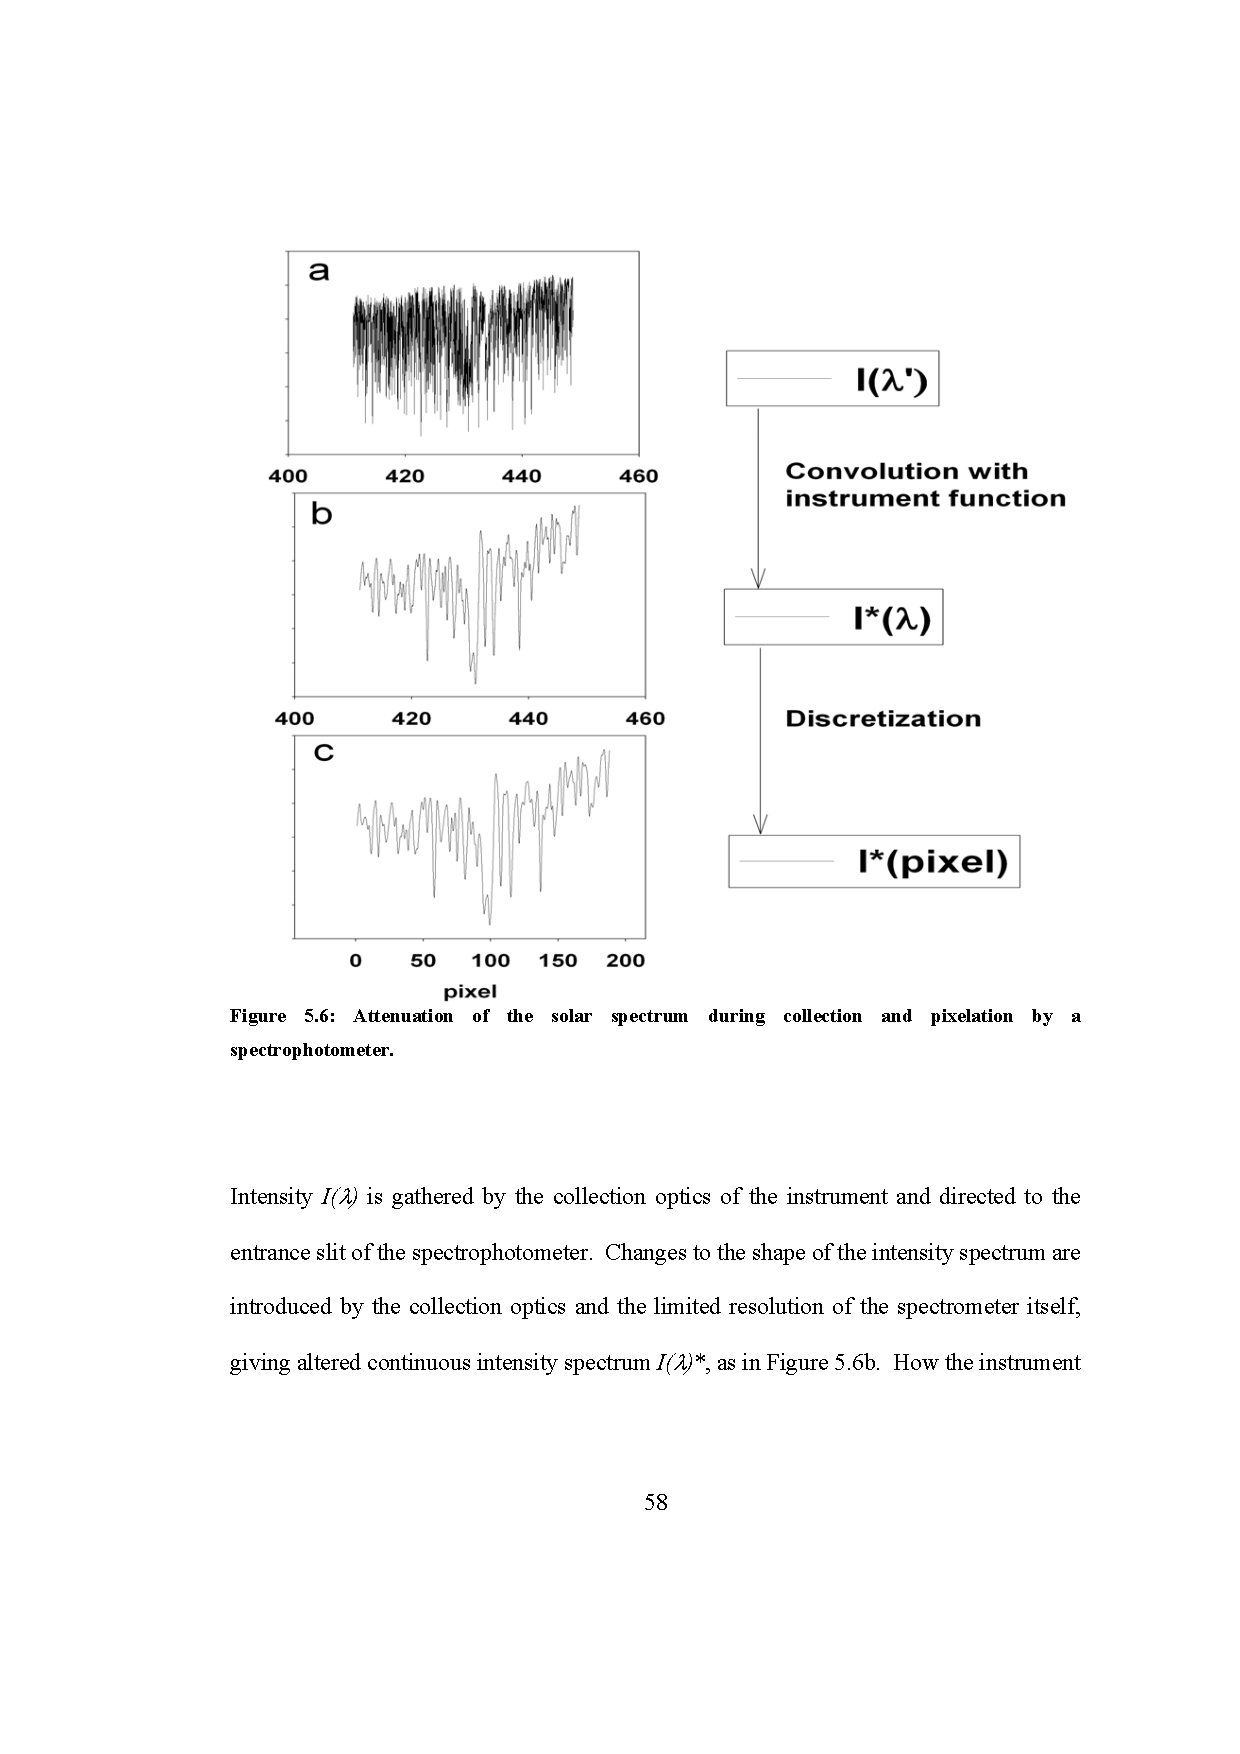
\includegraphics[clip,%
    trim=3cm 13.1cm 3cm 3cm,%
    width=.8\textwidth]{img/pdf/beekman_conditioning.pdf}
    \caption{Before being used in \gls{DOAS} calculations, literature
    trace gas cross section spectra must undergo a conditioning process
    to make sure they are compatible with the current experiment's
    instruments. Figure adapted from~\cite{Beekman2010}}
    \label{fig:cross_section_conditioning}
\end{figure}

\subsection{Spectral Calibration}%
\label{sub:spectral_calibration}

One other small but important incorrection that can bias results is the
lack of proper calibration between cross sections and collected spectra.
Figure~\ref{fig:conditioned_cross_section_discrepancy} shows how can a
conditioned cross section present slight wavelength related
discrepancies.

\begin{figure}[htpb]
    \centering
    \includegraphics[width=.8\textwidth]{img/png/calibration_differences.png}
    \caption{This figure, taken from~\cite{Beekman2010}, shows the difference
    between NO\textsubscript{2} cross sections. The red line comes from
    the literature, and has been conditioned to the experiment spectrometer.
    The blue line was actually collected with that device. The slight
    discrepancies that can be observed are calibration defects.}
    \label{fig:conditioned_cross_section_discrepancy}
\end{figure}

These small nonconformities are caused not only because both types of
data were captured by different spectrometers, but also because
conditions most certainly changed. This means that situations in which
calibration must be handled with care are the norm. This is done by
running an iterative process that makes slight adjustments to the
function mapping wavelength to pixel number, as explained in the next
few paragraphs.

The light that enters the spectrometer is scattered by the diffraction
grating before reaching the device's sensor, which is divided into
pixels. These pixels have a well defined and finite width. At the centre
of each one of them, the signal's intensity can be described by
Equation~\ref{eq:pixel_mapping_integral}, in which $I$ is the intensity,
$i$ the pixel number and $\lambda$ the wavelength.

\begin{equation}
    \centering
    I(i) = \int_{\lambda(i)}^{\lambda(i+1)} I(\lambda)d{\lambda}
    \label{eq:pixel_mapping_integral}
\end{equation}

The expression in Equation~\ref{eq:pixel_mapping_integral} assumes that
the signal has been conditioned properly, as described in
Section~\ref{sub:cross_section_conditioning}, through the convolution of
the cross section data with the instrument function and adequate
discretisation. The smaller $\Delta \lambda = \lambda(i+1)-\lambda(i)$,
the finer the instrument's resolution. This is, of course, inherent to
the system and cannot be changed. What can and should be changed during
analysis is the central wavelength assigned to each pixel. This
assignment is in fact what constitutes the instrument's calibration.

The most common way of conducting said calibration is by introducing a
polynomial describing wavelength to pixel relationship. This polynomial
is the wavelength-pixel mapping function, and can be written as in
Equation~\ref{eq:wavelength_pixel_function}.

\begin{equation}
    \centering
    \lambda(i) = \sum_{k=0}^{q} \gamma_{k} \cdot i^k
    \label{eq:wavelength_pixel_function}
\end{equation}

In Equation~\ref{eq:wavelength_pixel_function}, $\gamma_{k}$ determines
how the pixels are mapped to the wavelength ($\lambda$), and the type of
mapping effect depends on $k$. Changing $\gamma_{0}$ shifts the signal
left or right; changing $\gamma_{1}$ introduces linear distortions to
the pixel mapping, i.e., stretching or squeezing of the signal. One can
fit this polynomial up towards $k=\infty$, in theory, but normal
spectrometer calibrations are only run up to the second or third degree.
The Avantes spectrometers that were used in this dissertation are
factory-calibrated to a fourth order polynomial. 

The non-linear portion of the \gls{DOAS} algorithm, described in
Section~\ref{sec:doas}, is indeed a wavelength calibration. However, it
is important to previously calibrate every spectral signal before
actually running the \gls{DOAS} fitting process. This is because the
types of optimisation algorithm used in this technique, such as
Levenberg--Marquardt, tend to find local minima or to not converge if
there is significant misalignment between the spectra.

For passive applications using the sun as the light source, one can use
a high resolution solar spectrum (see Figure~\ref{fig:kurucz}), and the
Fraunhofer bands in it (which have a very well defined wavelength that
can be used as ground truth) to align the various spectra. For active
applications, one can use the light source's own spectrum, either
provided by the manufacturer or previously collected in the absence of
atmospheric or other effects.


\begin{figure}[htpb]
    \centering
    %left bottom right top
    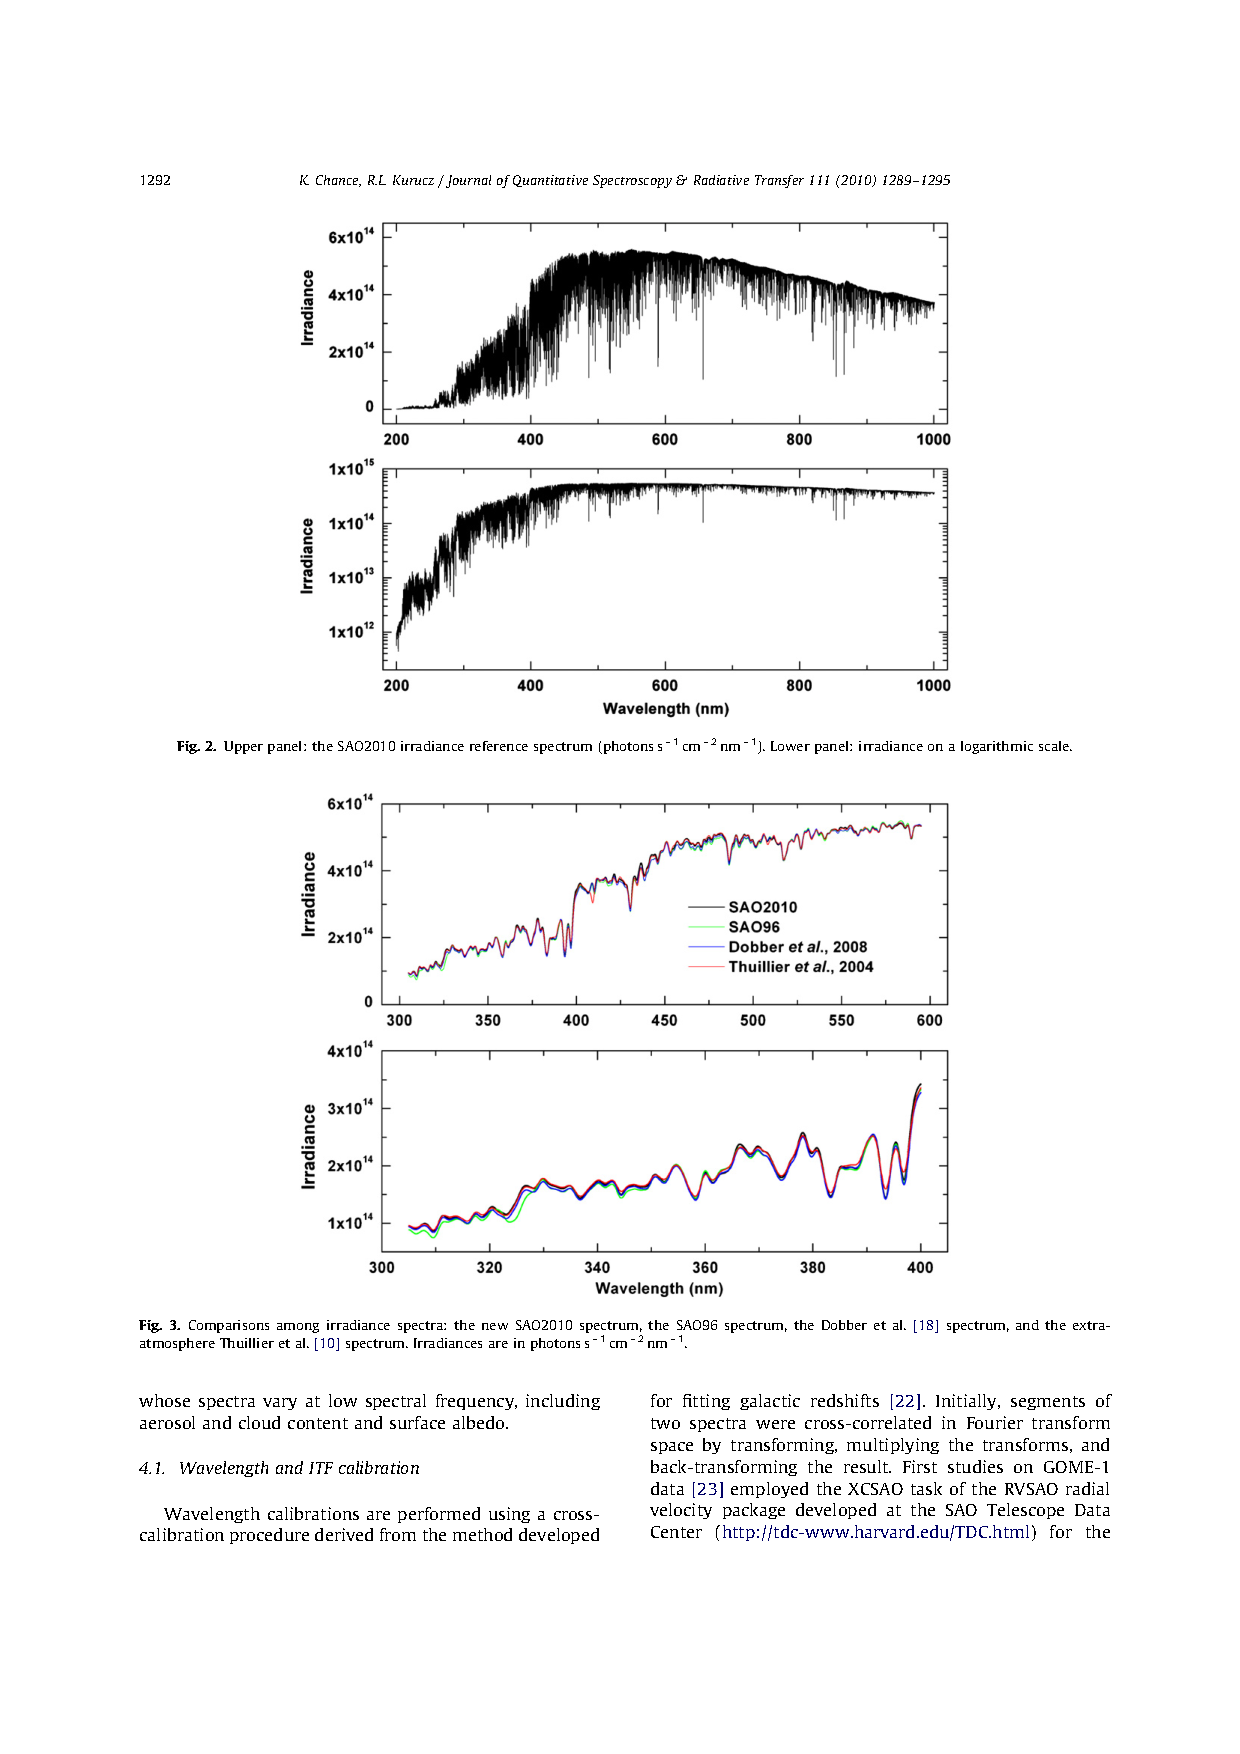
\includegraphics[clip,%
    trim=5.5cm 22cm 4.5cm 3.5cm,%
    width=\textwidth]{img/pdf/chance_kurucz.pdf}
    \caption{High resolution solar spectrum commonly used to calibrate
    the various spectral signals in \gls{DOAS}
    experiments~\cite{Chance2010}.}
    \label{fig:kurucz}
\end{figure}

